\documentclass[class=ctexart,crop=false,fleqn]{standalone}

\usepackage{amsmath,amssymb,enumitem,empheq,tkz-euclide,
diagbox,wrapfig,pgfplots}
\pgfplotsset{compat=newest}
\renewcommand\parallel{\mathrel{/\mskip-2.5mu/}}

\newcommand\px{\mathrel{/\mkern-5mu/}}  %平行
\newcommand\pxeq{\mathrel{\vcenter{     %平行且等于
\ialign{\hfil##\hfil\crcr
$\scriptstyle\px\!$\crcr
\noalign{\nointerlineskip\vskip1pt}$=$\crcr}}}}

%\setCJKmainfont{SimSun}       %设置西文字体为times new roman
%\setCJKsansfont{SimSun}             %设置中文字体为宋体
%\setCJKmonofont{STKaiti}
%\setsansfont{TeX Gyre Termes}            %设置typewriter family中文字体为楷体
%\setmonofont{TeX Gyre Termes}

\usetikzlibrary{calc,intersections,through,backgrounds,patterns}
\newcounter{para}
\newcommand\mypara{\par\refstepcounter{para}\thepara.\space}%设置typewriter family西文字体为times new roman
\newcommand*\circled[1]{\tikz[baseline=(char.base)]{
            \node[shape=circle,draw,inner sep=1.3pt] (char) {#1};}}
\begin{document}
点到直线距离公式推导( $AB$ 均不为0 ):\\
\begin{enumerate}[label=法\chinese*:]
  \item 面积法\\
    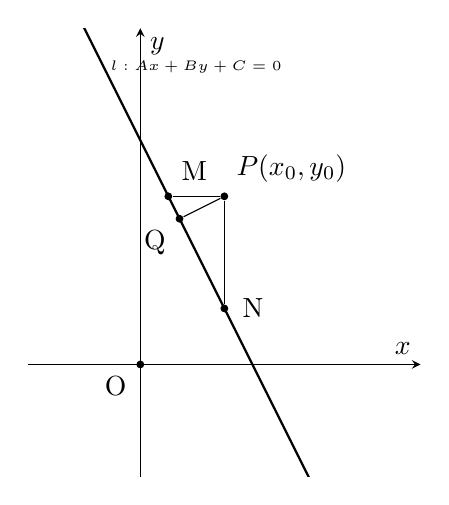
\begin{tikzpicture}
      \begin{axis}[
        unit vector ratio*=1 1 1 ,
        axis x line = middle,
        axis y line = middle,
        xlabel      = {$x$},
        ylabel      = {$y$},
        xmin=-2, xmax=5,
        ymin=-2, ymax=6, 
        ytick=\empty ,
        xtick=\empty ,
        legend pos=outer north east,
        legend style={draw=none},
      ]
        \addplot +[no markers,
          thick,
          black,
        ]{-2*x+4};
        \node[label={[label distance=0.005cm]60:{$P(x_0,y_0)$}},circle,fill,inner sep=1pt] (P) at (axis cs:1.5,3) {};
        \node[label={[label distance=0.05cm]0:{N}},circle,fill,inner sep=1pt] (N) at (axis cs:1.5,1) {};
        \node[label={[label distance=0.03cm]60:{M}},circle,fill,inner sep=1pt] (M) at (axis cs:0.5,3) {};
        \node[label={[label distance=0.005cm]210:{Q}},circle,fill,inner sep=1pt] (Q)  at ($(M)!(P)!(N)$) {};
        \node[label={[label distance=0.005cm]210:{O}},circle,fill,inner sep=1pt] (O)  at (axis cs:0,0) {};
        \node [coordinate,label={[font=\tiny]0:$l:Ax+By+C=0$}] (node1) at (axis cs:-0.7,5.3){};
        \draw (M)--(P)--(N);
        \draw (P)--(Q);
      \end{axis}
    \end{tikzpicture}\\
    作 $PM\perp y$轴交 $l$于 $M$,\\
    作 $PN\perp x$轴交 $l$于 $N$.\\
    则:$M(x_M,y_0),N(x_0,y_N)$满足直线方程
    \begin{flalign}
      &\left\{
        \begin{aligned}
          & Ax_M+By_0+C=0\\
          &Ax_0+By_N+C=0          
        \end{aligned}
      \right.
    \end{flalign}
    $x_M=\frac{-By_0-C}{A}$,$y_N=\frac{-Ax_0-C}{B},\\
    PM=\frac{Ax_0+By_0+C}{B},PN=\frac{Ax_0+By_0+C}{A},\\
    MN=(Ax_0+By_0+C) \sqrt{(\frac{1}{A})^2+(\frac{1}{B})^2}.$\\
    故关于点到直线距离 $PQ$,有:\\
    $\begin{aligned}[t]
      S_{\triangle PMN}&=PM \times PN=MN \times PQ\\
        \Rightarrow PQ&=\frac{PM \times PN}{MN} \\
      &=|\frac{(Ax_0+By_0+C)(Ax_0+By_0+C)}{AB(Ax_0+By_0+C) \sqrt{(\frac{1}{A})^2+(\frac{1}{B})^2}}|\\
      &=\frac{|Ax_0+By_0+C|}{\sqrt{A^2+B^2}}
    \end{aligned}$
  \item 交点法\\
    直线 $PQ \perp l,$
    故设 $PQ:Bx-Ay+D=0$.\\
    又 $P \in PQ \Rightarrow D=-Bx_0+Ay_0.$
    故垂足$Q(x,y)$满足:\\
    \[      \left\{
      \begin{aligned}
        & Ax+By+C=0\\
        &Bx-Ay-Bx_0+Ay_0=0          \\
      \end{aligned}
      \right. \]\\
      $\begin{aligned}
        &\circled{1} \times B-\circled{2} \times A:\\
        &ABx+B^2y+BC-ABx+A^2y+ABx_0-A^2y_0=0\\
        &(A^2+B^2)y=A^2y_0-ABx_0-BC\\
        &\Rightarrow y=\frac{A^2y_0-ABx_0-BC}{A^2+B^2}\\
        &\circled{1} \times A+\circled{2} \times B:\\
        &A^2x+ABy+AC+B^2x-ABy-B^2x_0+ABy_0=0\\
        &(A^2+B^2)y=B^2x_0-ABy_0-AC\\
        &\Rightarrow x=\frac{B^2x_0-ABy_0-AC}{A^2+B^2}
      \end{aligned}$\\
      则: $\begin{aligned}[t]
        PQ&=\sqrt{(x-x_0)^2+(y-y_0)^2}\\
        &=\sqrt{(\frac{A^2x_0+ABy_0+AC}{A^2+B^2})^2+(\frac{ABx_0+B^2y_0+BC}{A^2+B^2})^2}\\
        &=\frac{|Ax_0+By_0+C|}{A^2+B^2}\times \sqrt{A^2+B^2}\\
        &=\frac{|Ax_0+By_0+C|}{\sqrt{A^2+B^2}}
      \end{aligned}$\\
  \item 向量法\\
    $l$ 的一个方向向量为 $(-B,A)$ ,一个法向量 $\vec{n}$ 为 $(A,B)$\\
    $Q(x_1,y_1)$ 为 $l$ 上的任意一点\\
    则有 $Ax_1+By_1+C=0$ \\ 
    由向量内积公式,\\
    $\begin{aligned}[t]
      d=&|\overrightarrow {QP}||\cos<\overrightarrow{QP},\vec{n}>|\\
      =&\frac{|\overrightarrow{QP}  \cdot \vec{n}|}{|\vec{n}|}\\
      =&\frac{|(x_0-x_1,y_0-y_1)(A,B)|}{\sqrt{A^2+B^2}}\\
      =&\frac{|(Ax_0-Ax_1+By_-By_1)(A,B)|}{\sqrt{A^2+B^2}}\\
      =&\frac{|Ax_0+By_0+C|}{\sqrt{A^2+B^2}}\\
    \end{aligned}$\\
  \item 三角函数法\\
    记 $l$ 的倾角为 $\alpha$\\
    $M(x_M,y_0)$ , $RQ \perp y$ 轴,与 $l$ 交于 $M$ \\
    则: $x_M=\frac{n-By_0-C}{A}$\\
    $\begin{aligned}[t]
      &|x_M-x_0|=|\frac{Ax_0+BY_0+C}{A}|\\
      \text{又有:} &\frac{1}{sin^2\alpha}=tan^2\alpha+1\\
      &sin\alpha=\sqrt{\frac{1}{1+tan^2\alpha}}\\
      &sin\alpha=\sqrt{\frac{1}{1+(-\frac{B}{A})^2}}\\
      &sin\alpha=\frac{A}{\sqrt{A^2+B^2}}\\
      \text{故:} &d=|x_M-x_0||\sin\alpha|\\
      &d=|\frac{A(Ax_0+BY_0+C)}{A\sqrt{A^2+B^2}}|\\
      &d=\frac{|Ax_0+BY_0+C|}{\sqrt{A^2+B^2}}\\
    \end{aligned}$
\end{enumerate}

   


\end{document}